A compensation for the in image plane rotation of a face can be achieved by taking advantage of the symmetry of faces, namely that both eyes most often form a vector that is parallel to the horizon. After the extraction of such a vector one can easily find the rotation of the face.

The algorithm we use to locate the eyes is called the \textit{Circular Hough Transform} (CHT) which is a feature extraction technique for finding circles. The algorithm is popular and often used because of its robustness in noisy areas and tolerance for occlusion and varying illumination \cite{cht}. However there exits no specific manual on how to implement an algorithm based on CHT, a brief description of how it can be done is though included below.

TODO: fix the stuff below. Find a better source etc.

% https://www.cis.rit.edu/class/simg782/lectures/lecture_10/lec782_05_10.pdf

% http://docs.opencv.org/2.4/doc/tutorials/imgproc/imgtrans/hough_circle/hough_circle.html

The first step can be to define an accumulator array where \textit{votes} can be stored. More votes on a pixel increases the likelihood of it being a center point for a circle. The foreground pixels of high gradients are then chosen to act as candidate pixels which are allowed to cast \textit{votes} in the accumulator array. The candidate pixels then vote in a circle pattern around them, which is illustrated by Figure \ref{fig:CHT}.

\begin{figure}[H]
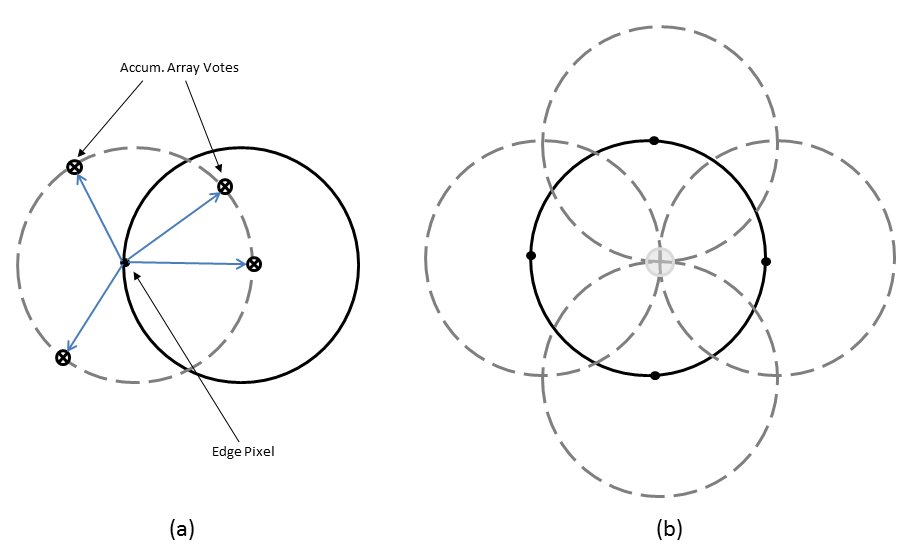
\includegraphics[scale=0.4]{img/fd/accarray.png}
\caption{CHT voting pattern to estimate the center of the circle.}
\label{fig:CHT}
\end{figure}

The second step is to estimate a center point. The position votes from the candidate pixels belonging to an image circle tend to accumulate at the center of the circle. Therefore, the center of the circle is estimated by detecting the peaks in the accumulator array, where the votes are stored.


